\documentclass{amsart}
\usepackage[ruled,vlined]{algorithm2e}
\usepackage{amsmath}
\usepackage[margin=1in]{geometry}
\DeclareMathOperator*{\argmax}{arg\,max}
\DeclareMathOperator*{\argmin}{arg\,min}
\usepackage{ifpdf}
\usepackage{url}
\usepackage{graphicx}
\usepackage{float}
\usepackage{amsfonts}
\title{Project 4 \\ Logistic Regression and Adaline Networks}
\author{David Atlas}
\begin{document}
    \begin{abstract}
    This paper will introduce two parametric algorithms for
    classifying linearly seperable classes. Logistic Regression
    applies a log-odds transformation to the target class to make predictions
    on the likelihood of a instance belonging to a class.
    An Adaline Network attempts to predict the class value (0 or 1) using
    a linear transformation. Both algorithms are trained using gradient
    descent. This paper will also apply both classifiers to 5 real
    world datasets. It is expected that the algorithms will perform
    similarly on real world data, as they are both able to find linear
    discriminants, and thus have similar model capacity. Real-world experiments
        indicate that performance tends to be similar between the two algorithms,
        and both outperform baselines on the datasets used.

    \end{abstract}

    \maketitle

    \section{Problem Statement \& Hypothesis}
    This paper introduces techniques to find a linear discriminant
    between classes, based on a set of attributes about the classes.
    The parameters of the linear discriminant are learned via a
    gradient descent type algorithm. Because both techniques are linear,
    it is expected that they perform comparably on any given problem, as neither has an
    advantage in capacity.

    It is expected that both techniques will not be able to learn
    classifications on non-linearly seperable problems without
    first transforming features. In Figure~\ref{nonseperable_classes},
    such a problem is shown.
    \begin{figure}[H]
        \centering
        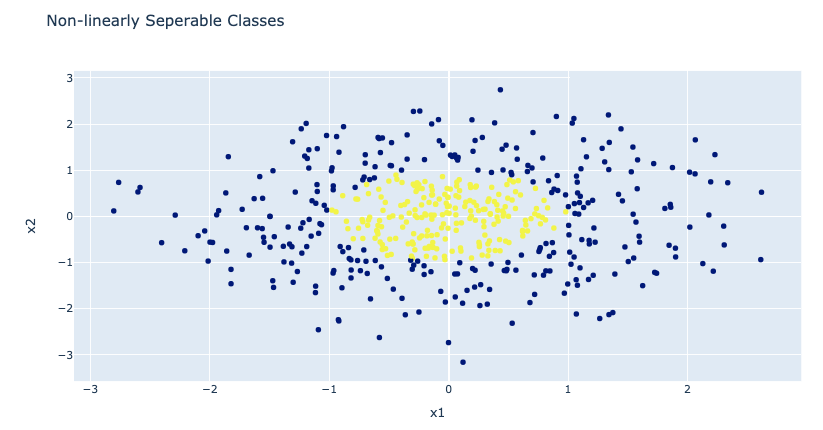
\includegraphics[width=.9 \textwidth]{non-seperable.png}
        \label{nonseperable_classes}
        \caption{In the figure above, the yellow class cannot be seperated from the
        blue class via a single linear discriminant. In such a situation,
        the linear discriminant methods would be expected to perform
        poorly on a classification task.
        }
    \end{figure}
    As such the classification accuracy of the algorithms will be inline with
    the proportion of instances that are linearly seperable. Problems that are
    mostly linearly seperable, but where labels are noisy, will have accuracy proportional
    to the degree of noise.

    Because the algorithms both involve linear transformations of the
    features, they do not natively handle any discrete-multivalued attributes.
    Such inputs must be transformed to one-hot encodings.

    The algorithms do not have capacity to identify interactions between
    input features. All such interactions must be identified manually and encoded
    as a seperate input. Likewise,
    non-linear relationships between features and the class
    will not be learned by the algorithm.

    Both techniques are relatively efficient to train, although the
    gradient descent algorithm may not converge if problems are not linearly
    seperable, and the learning rate of the algorithm has a significant impact on convergence.

    \section{Description of Algorithm}
    \subsection{Logistic Regression}
    \subsubsection*{Discriminant Development}
    The logistic regression algorithm creates a linear discriminant between two classes. Suppose
    $k$ classes $(C_1, \cdots, C_k)$ exist.
    The logistic regression classifier seeks to calculate
    \begin{align}
        \textrm{logit} ~P(C_k \mid x) = \log \frac{P(C_1 \mid x)}{1 - P(C_1 \mid x)},
        \label{logit_lr}
    \end{align}
    or the probability that instance $x$ belongs to class $C_k$ given the attributes of instance
    $x$.

    Given Equation~\ref{logit_lr} and applying Bayes' Rule, it follows that
    \[
        \log \frac{P(C_k \mid x)}{1 - P(C_k \mid x)} =
        \log \frac{P(x \mid C_k)}{1 - P(x \mid C_k)} + \log \frac{P(C_k)}{1 - P(C_k)}.
    \]
    This will be expressed as a linear discriminant:
    \begin{align}
         \log \frac{P(x \mid C_k)}{1 - P(x \mid C_k)} + \log \frac{P(C_k)}{1 - P(C_k)} = w_k^T x + w_{k_0}.
        \label{lin_discriminant}
    \end{align}
    Using a bit of algebra, Equation~\ref{lin_discriminant} can be turned into \[
        P(C_k \mid x) = \frac{\exp{(w_k^T x + w_{k_0})}}{\sum_{j=1}^K \exp{(w_j^T x + w_{j_0})}},
    \]
    where the denominator is the sum over all of the class discriminants outputs. This normalizes
    the output for each class relative to the likelihoods predicted by the other classes.


    Mathematically, this implies that
    \begin{align*}
        \lim_{w_k^T x + w_{k_0} \to +\infty} P(C_k \mid x) &= 1 \\
        \lim_{w_k^T x + w_{k_0} \to -\infty} P(C_k \mid x) &= 0.
    \end{align*}

    \subsubsection*{Learning Parameters}
    An appropriate loss function for logistic regression is cross-entropy loss. This is defined
    as
    \[
        \textrm{E}(w_k^T \mid x) = -\sum_{t} r^t \log y^t + (1 - r^t)\log (1 - y^t),
    \]
    where $y^t = w_k^T x^t$ (for notational simplicity, it is assumed that the first column of $X$ is a vector of ones, acting
    as the intercept). $r^t$ is the actual class of the instance.

    Therefore, the gradient of the loss function with respect to the model parameters is
    \[
        \frac{dE}{dw_k} = - \sum_t (r^t - y^t) x^t.
    \]
    This will be used in the gradient descent algorithm as the following update rule:
    \begin{align*}
        \Delta w_k &= -\eta \frac{dE}{dw_k} = \eta \sum_t (r^t - y^t) x^t \\
        w^{n+1}_k &= w^{n}_k + \Delta w^{n}_k
    \end{align*}
    This process is repeated iteratively until some convergence criteria is met, or a maximum number
    of iterations is exceeded.

    \subsubsection*{Prediction}
    At prediction time, the outputs of each of the $k$ discriminants are calculated, and the largest one is chosen.
    Because the outputs are normalized by the outputs of all of the other classes, the class that has the largest
    value is the most likely class for that instance.

    \subsection{Adaline Network}
    \subsubsection*{Training}
    The Adaline Network unit is quite similar to the logistic regression model. A linear
    discriminant is estimated via gradient descent. The primary difference is that rather than
    applying the logistic function to the output of the linear transformation, the Adaline Network
    tries to minimize the squared distance between its network outputs and the correct value.

    To train the network, the squared error loss function is used:
    \[
        E(w, x^t) = \sum_{t}(w^T x^t - r^t)^2,
    \]
    where $w_k$ are the weights of the network (as above, assuming the first element of $x^t$ is a 1 representing the
    intercept), and $r^t \in \{0, 1\}$ is the correct label. Next, the gradient of the loss function  with respect to
    $w^T$ must be calculated:
    \[
        \frac{dE}{dw} = \sum_t (w^T x^t - r^t)x^t.
    \]
    This leads to the following update rule:

    \begin{align*}
        \Delta W &= \eta (r^t - w^T x^t) x^t \\
        W^{n+1} = W^n + \Delta W^{n}
    \end{align*}

    \subsubsection*{Prediction}
    At prediction time, the output of the network is discretized to produce a class, with values above .5 taken
    as a 1, and those below .5 as a zero. The raw output of the network can be used as a proxy for the prediction probability,
    which is leveraged in multiclass problems, where 1 vs. $k$ classifiers are trained, and the class with the
    largest probablity is chosen.

    \section{Experimental Approach}
    The algorithms described above were applied to 5 real-world problems. As neither of the algorithms can
    handle null-values, those values were either dropped or transformed into one-hot encoded variables. Likewise,
    multi-valued discrete features are transformed to one-hot encoded variables.

    Each of the datasets undergo feature transformation to scale everything to $[-1,1]$, where
    all values are divided by the maximum absolute value in the column.

    For each dataset, the algorithms are measured by their accuracy on the classification problem. They are also compared
    to a naive baseline model that predicts the mode over the training data.

    Stratefied 5-Fold cross-validation is used to get a better estimate of the performance of each classifier on
    various out-of sample portions of the data.

    \section{Experiment Results}
    \subsection{Breast Cancer Dataset}
    The Breast Cancer dataset\cite{cancerdataset} involves classifying tumors as malignant or benign based
    on characteristics of the tumors. This is a simple two-class problem, with continuous valued inputs, and
    so no data transformation is needed. The features are scaled using the max-scaler described above.
    The results of the experiments are shown in Table~\ref{breast_results}.
    \begin{table}
    \begin{tabular}{lc}
    Algorithm & Average Accuracy \\
    \hline
    Naive Baseline & 65.0\% \\
    Logistic Regression & 96.5\% \\
    Adaline & 95.5\%
    \end{tabular}
    \caption{Breast Cancer dataset experiment results.}
    \label{breast_results}
    \end{table}

    \subsection{Glass Dataset}
    The Glass Dataset\cite{glassdataset} involves classifying the source of
    broken glass based on characteristics about the glass. This is a multi-class
    classification problem, and so a one-vs-all approach is used for the
    Adaline Network. Logistic regression handles that scenario naturally.
    The features are scaled using the max-scaler approach from above.
    The results can be found in Table~\ref{glass_results}.
\begin{table}[H]
    \begin{tabular}{lc}
    Algorithm & Average Accuracy \\
    \hline
    Naive Baseline & 35.5\% \\
    Logistic Regression & 44.5\% \\
    Adaline & 50.5\%
    \end{tabular}
    \label{glass_results}
        \caption{Glass dataset experiment results.}
    \end{table}

    \subsection{Iris Dataset}
    The Iris Dataset\cite{irisdataset} presents a classification
    problem in which the species of iris flower must be classified based
    on attributes about the plant. All features are continuously
    valued, and so no encodings are needed there, but all features are transformed
    using the max-scaler. This is a multi-class problem, and so
    a one-vs-all approach is used for the Adaline Network. The results are
    shown in Table~\ref{iris_results}
    \begin{table}[H]
    \begin{tabular}{lc}
    Algorithm & Average Accuracy \\
    \hline
    Naive Baseline & 33.3\% \\
    Logistic Regression & 85.3\% \\
    Adaline & 96.6\%
    \end{tabular}
    \label{iris_results}
        \caption{Iris dataset experiment results.}
    \end{table}

    \subsection{Soybean Dataset}
    The soybean dataset\cite{soybeandataset} has a classification
    problem in which the type of rot is classified based on
    features about the beans. The features are all discrete
    valued, and so all columns are one-hot encoded. The results
    are shown in Table~\ref{soybean_results}.
    \begin{table}[H]
    \begin{tabular}{lc}
    Algorithm & Average Accuracy \\
    \hline
    Naive Baseline & 36\% \\
    Logistic Regression & 100\% \\
    Adaline & 100\%
    \end{tabular}
    \label{soybean_results}
    \caption{Soybean dataset experiment results.}
    \end{table}

    \subsection{House Votes Dataset}
    The house voting dataset\cite{housedataset} involves a classification
    problem where the party of the voter is predicted
    based on their votes. All of the features are one-hot encodings.
    Null values are encoded as their own boolean values.
    The results of the experiments are shown in Table~\ref{house_votes_results}.
    \begin{table}[H]
    \begin{tabular}{lc}
    Algorithm & Average Accuracy \\
    \hline
    Naive Baseline & 61.4\% \\
    Logistic Regression & 94.7\% \\
    Adaline & 95.4\%
    \end{tabular}
    \label{house_votes_results}
    \caption{House Votes dataset experiment results.}
    \end{table}



\bibliographystyle{plainurl}
\bibliography{biblio}


\end{document}